\documentclass[10pt,a4paper]{article}
\usepackage[utf8]{inputenc}
\usepackage{amsmath}
\usepackage{amsfonts}
\usepackage{amssymb}
\usepackage{listings}
\usepackage{graphicx}
\graphicspath{ {../img/} }
\author{Gradey Cullins}
\title{Assignment 6}
\begin{document}
\maketitle

\section*{Explanation of Code}
The submitted code contains one script called \emph{main.m}. The script is divided into two sections. \\

\noindent
The first section solves and plots the 1-D solution to the heat equation. \\

\noindent
The second section contains the Laplace solution and plots the mesh grid for the requested sizes from the homework specification.

\section{}

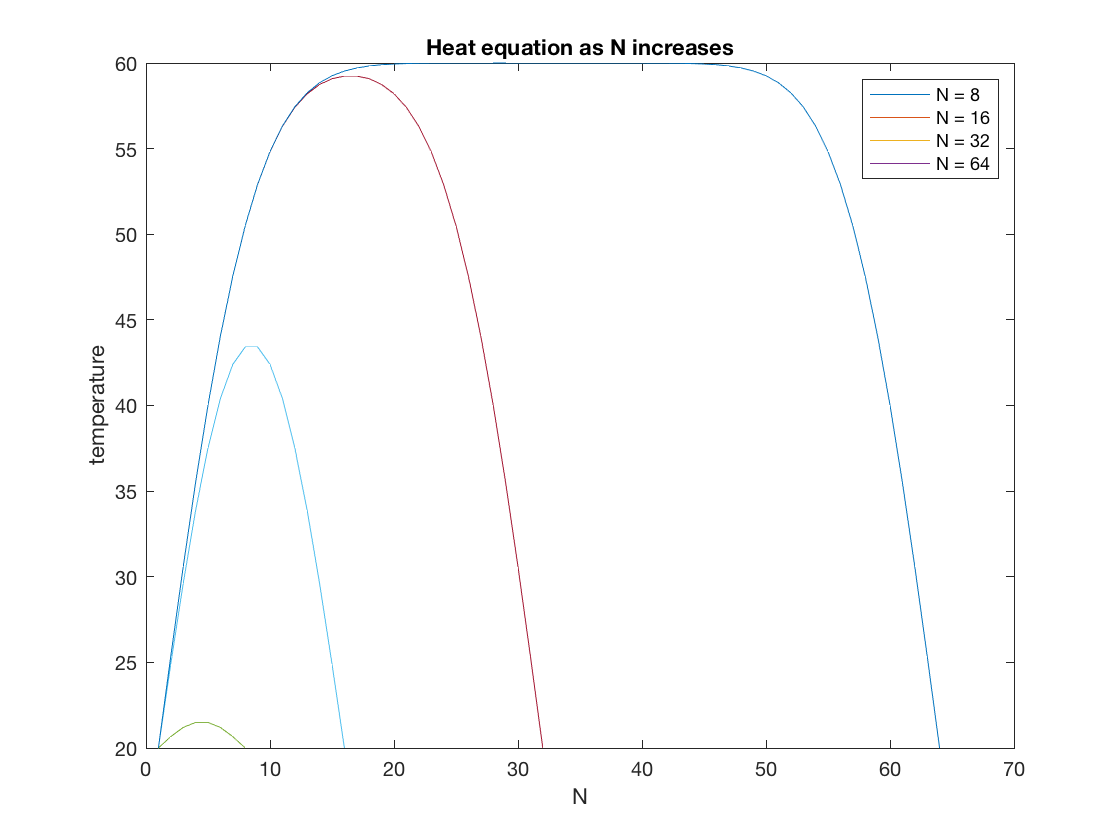
\includegraphics[scale=0.2]{fig_1.png}
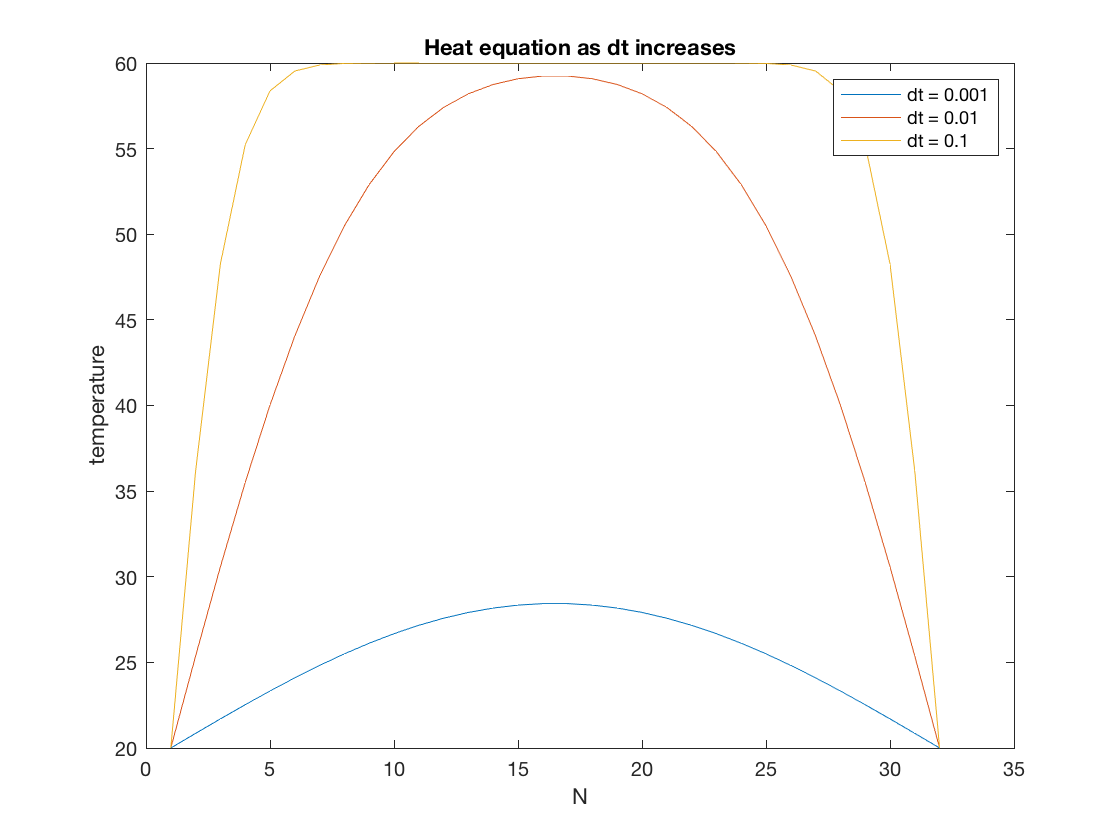
\includegraphics[scale=0.2]{fig_2.png}

\noindent
As N increases, so does the maximum temperature on the y axis. From figure 1, it is clear that the solution takes its most reasonable form when N reaches 64, as here the plot hits the ceiling and remains largely constant until near the end of x axis. Further, the reach of the x values increases as N increases. \\

\noindent
As dt increases, so does the maximum temperature on the y axis, similar to the first plot. One difference between the two plots is the variable dt plot shows that the maximum x value is the same across multiple runs, probably due to a constant N. Additionally, as dt increases, the rate or steepness of the plot decreases. Therefore the steepness is inversely proportional to the change in time dt.


\section{}

\subsection*{i}
The true function u is defined by: \\
$ u_{true}(x,y) = sin(\pi * x)e^{(-\pi * y)} $ \\
The second derivative is: \\
$ \pi^2 * (-e^{-\pi * y}) * sin(\pi * x) $ \\

\noindent
My code for problem 2 only prints out the resulting matrix \emph{p}. In order to calculate the error norm, I would norm the absolute value of the result of subtracting my answer matrix with the matrix resulting from using the true second derivative of the function u.

\subsection*{ii}

I modified the submitted Laplace code to have a convergence condition dependent on the condition that: \\

\noindent
$ (c / (1 - c))* abs(x_k+1 - x_k)  \leq tol$ \\

\noindent
I chose my tolerance such that the number of iterations was reasonably low but the error was also reasonably low and additionally avoided issues with numerical instability.

\end{document}
